%% Copernicus Publications Manuscript Preparation Template for LaTeX Submissions
%% ---------------------------------
%% This template should be used for copernicus.cls
%% The class file and some style files are bundled in the Copernicus Latex Package which can be downloaded from the different journal webpages.
%% For further assistance please contact the Copernicus Publications at: publications@copernicus.org
%% http://publications.copernicus.org


%% Please use the following documentclass and Journal Abbreviations for Discussion Papers and Final Revised Papers.


%% 2-Column Papers and Discussion Papers
\documentclass[esurf, manuscript]{copernicus}





%% \usepackage commands included in the copernicus.cls:
%\usepackage[german, english]{babel}
%\usepackage{tabularx}
%\usepackage{cancel}
%\usepackage{multirow}
%\usepackage{supertabular}
%\usepackage{algorithmic}
%\usepackage{algorithm}
%\usepackage{amsthm}
%\usepackage{float}
%\usepackage{subfig}
%\usepackage{rotating}


\begin{document}

\title{A lattice grain model of hillslope evolution}


% \Author[affil]{given_name}{surname}

\Author[1]{Gregory E.}{Tucker}
\Author[]{}{}
\Author[]{}{}

\affil[1]{Cooperative Institute for Research in Environmental Science (CIRES) and Department of Geological Sciences, University of Colorado, Boulder, CO 80305 USA}
\affil[]{ADDRESS}

%% The [] brackets identify the author with the corresponding affiliation. 1, 2, 3, etc. should be inserted.



\runningtitle{TEXT}

\runningauthor{TEXT}

\correspondence{NAME (EMAIL)}



\received{}
\pubdiscuss{} %% only important for two-stage journals
\revised{}
\accepted{}
\published{}

%% These dates will be inserted by Copernicus Publications during the typesetting process.


\firstpage{1}

\maketitle



\begin{abstract}
TEXT
\end{abstract}



\introduction  %% \introduction[modified heading if necessary]

Hillslopes take on a rich variety of forms. Their profile shapes may be convex-upward, concave-upward, planar, or some combination of these. Some slopes are completely mantled with soil, whereas others are bare rock, and still others draped in a discontinuous layer of mobile regolith. The processes understood to be responsible for shaping them are equally varied, ranging from disturbance-driven creep to dissolution to large-scale mass movement events.

Considerable research has been devoted to understanding the evolution of soil-mantled slopes that are primarily governed by disturbance-driven creep, such as down-slope soil transport by biotic and abiotic soil-mixing processes. As a result, the geomorphology community has mathematical models that account well for observed slope forms and patterns of regolith thickness \citep[e.g.,][]{roering2008well}. Furthermore, stochastic-transport theory provides a mechanistic link between the statistics of particle motion, the resultant average rates of downslope transport, and the emergence of convex-upward, soil-mantled slope forms \citep{culling,furbish}.

One gap that remains, however, lies in understanding steep, rocky slopes. ``Rocky'' implies slopes that lack a continuous soil cover; here, transport laws that assume the existence such a cover no longer apply. ``Steep'' implies angles approaching or exceeding the effective angle of repose for loose, granular material, so that ravel may be an important transport mode \citep[e.g.][]{gabet,lamb,stock} and particles have the potential to fall as soon as they are released from bedrock. This type of relatively fast, long-distance transport does not fit comfortably in the framework of standard diffusion-based models of hillslope soil transport, which derive from an underlying assumption that the characteristic length scale of motion is short relative to the length of the slope [REFS].

Rocky slopes are rarely completely barren. More commonly, they have a patchy cover of loose scree, which could either retard rock weathering by shielding the rock surface from moisture or temperature fluctuations, or enhance it by trapping water and allowing limited plant growth. A discontinuous cover does not fit easily within the popular exponential-decay regolith-production models [SOME REF], which assume an essentially continuous soil mantle.

An additional issue, which pertains to both rocky and soil-mantled slopes, is the connection between sediment movement at the scale of individual ``motion events,'' and the resulting longer-term average sediment flux, which forms the basis for continuum models of hillslope evolution. Recent theoretical and experiment work has begun to forge a mechanistic connection between these scales [REFS Furbish especially, building on earlier work by Culling]. However, the community's resources for computational analysis of particle-level dynamics remain limited [REFS], lagging behind developments in the understanding of fluvial sediment transport [REFS Schmeeckle etc.].

To further our understanding of how grain-level weathering and transport processes translate into hillslope evolution, both for hillslopes in general and rocky slopes in particular, it would be useful to have a computational framework with which to conduct experiments. Ideally, such a framework should be sophisticated enough to capture the essence of weathering and granular mechanics, while remaining simple enough to involve only a small number of parameters and providing reasonable computational efficiency.

Our aim in this paper is to describe one such computational framework, test whether it is capable of reproducing commonly observed hillslope-profile forms, and examine how its parameters relate to the bulk-behavior parameters used in conventional continuum models of soil creep and regolith production. The model uses a pairwise, continuous-time stochastic (CTS) approach to combine a lattice-grain model [REFS] with rules for stochastic bedrock-to-regolith conversion (``weathering'') and disturbance of surface regolith particles.

We begin with ... [outline sections of the paper]







\section{Model Description}

The model combines a cellular automaton representation of granular mechanics with rules for weathering of rock to soil and for episodic disturbance of soil. Cellular automata are widely used in the granular mechanics community, because they can represent the essential physics of granular materials at a reasonably low computational cost \citep{REFS}. Because the principles are often to similar to those of lattice-gas automata in fluid dynamics \citep[e.g.,][]{}, cellular automata for granular mechanics are sometimes referred to as lattice-grain models (LGrMs).

\subsection{CTS Lattice-Grain Model}

Our approach starts with a two-dimensional continuous-time stochastic (``CTS'') lattice-grain model. The model is described in detail by \citet{tucker2016celllab}; here we present a only brief overview of its rules and behavior. The framework is based on the pairwise method developed by Narteau and colleagues \citep{REFS} and applied to problems as diverse as eolian dune dynamics and the core-mantle interface.

In the CTS Lattice-Grain Model, the domain consists of a lattice of hexagonal cells. Each cell is assigned one of eight states (Table~\ref{statetable}). These states represents the nature and motion status of the material: state 0 represents fluid, states 1--6 represent a grain moving in one of the six lattice directions, and state 7 indicates a stationary grain. For purposes of modeling hillslope evolution, we add an additional state (8) to represent rock. Figure~\ref{lattice} illustrates these states, with an example of a single transition in which a falling grain switches places with the fluid cell below it.

%t
\begin{table}[t]
\caption{States in the lattice grain hillslope model.}
\begin{tabular}{cl}
\tophline
State & Description \\
\middlehline
0 & Fluid \\
1 & Moving upward \\
2 & Moving up and right \\
3 & Moving down and right \\
4 & Moving down \\
5 & Moving down and left \\
6 & Moving up and left \\
7 & Resting \\
8 & Rock \\
\bottomhline
\label{statetable}
\end{tabular}
\end{table}

%f
\begin{figure*}[t]
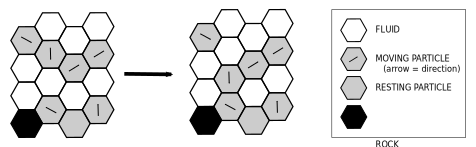
\includegraphics[width=12cm]{Figures/lattice_transition_illustration.pdf}
\caption{Example of a four-by-four lattice, illustrating the eight states in the lattice-grain hillslope model and including an example transition in which a falling grain trades places with the fluid cell below it.}
\label{lattice}
\end{figure*}

Like other lattice-grain models, the CTS Lattice-Grain Model is designed to represent, in a simple way, the motion and interaction of an ensemble of grains in a gravitational field. The physics of the material are represented by a set of transition rules, in which a given adjacent pair of states is assigned a certain probability per unit time of undergoing a transition to a different pair. For example, consider a vertically aligned pair of cells in which the top cell has state 4 (moving downward) and the bottom cell state 0 (empty/fluid). Downward motion (falling) is represented by a transition in which the two states switch places (Figure~\ref{lattice}).

% OK, SO NEED TO GET RID OF THE ELASTIC FIGURE, EXCEPT MOTION AND LEGEND, WHICH COULD BE ADDED TO THE FRICTIONAL FIGURE

%Elastic collisions are represented by a set of rules in which two adjacent grains that are converging have a given probability per unit time of rebounding and changing their directions. These rules are similar to the collision rules used in deterministic lattice-gas automata, with the main difference being that they account for the stochastic nature of transition events. 
We assume that biophysical disturbance events such as the growth of roots and burrowing by animals, and the settling motions that follow, tend to impart low kinetic energy, with ``low'' defined as ballistic displacement lengths that are short relative to hillslope length and comparable to or less than the characteristic disturbance-zone thickness. We view such motions as being dominated by frictional dissipation rather than by transfer of kinetic energy by elastic impacts. This view is similar to the reasoning of \citet{furbish2009statistical} that the mean-free-path of mobile grains will typically be short relative to hillslope length, scaling with the grain radius and particle concentration. For this reason, unlike the lattice-grain model of \citet{tucker2016celllab}, we consider here only inelastic collisions (Figure~\ref{frictional}). These inelastic (frictional) collisions are represented by a set of rules in which one or both colliding particles become stationary, representing loss of momentum and kinetic energy as a result of the collision. Gravity is represented by transitions in which a rising grain decelerates to become stationary, a stationary grain accelerates downward to become a falling particle, and a grain moving upward at an angle accelerates downward to move downward at an angle (Figure~\ref{gravity}). An additional rule allows for acceleration of a particle resting on a slope: a stationary particle adjacent to a fluid cell below it and to one side may transition to a moving particle. Importantly for our purposes, this latter rule effectively imposes an angle of repose at 30$^\circ$.

\begin{figure*}[t]
\includegraphics{Figures/lattice_grain_friction_rules.pdf}
\caption{Rules for motion and frictional (inelastic) collisions, illustrated here for one of the six lattice directions.}
\label{frictional}
\end{figure*}

\begin{figure*}[t]
\includegraphics{Figures/lattice_grain_gravity_rules.pdf}
\caption{Illustration of gravitational rules. The bottom row shows the ``falling on a slope'' rule, which effectively imposes a 30$^\circ$ angle of repose. Modified from \citet{tucker2016celllab}.}
\label{gravity}
\end{figure*}

One limitation of the CTS Lattice-Grain model is that falling grains do not accelerate through time; instead, they have a fixed transition probability that implies a statistically uniform downward fall velocity. This treatment is obviously unrealistic for particles falling in a vacuum, though it is consistent with a terminal settling velocity for grains immersed in fluid.

Tests of the CTS Lattice-Grain Model show that it reproduces several basic aspects of granular behavior \citep{tucker2016celllab}. For example, when gravity and friction are de-activated, the model conserves kinetic energy. When gravity and friction are active, the model reproduces some of the common behaviors observed with granular materials. For example, Figure~\ref{silo} illustrates a simulation of the emptying of a silo to form an angle-of-repose grain pile. For our purposes, what matters most is simply that the model captures, in a reasonable way, the response of particles on a slope to episodic disturbance events.

%f
\begin{figure*}[t]
\includegraphics[width=12cm]{Figures/lattice_grain_silo.pdf}
\caption{Lattice-grain simulation of emptying of a silo. Light-shaded grains are stationary; darker-shaded ones are in motion. From \citet{tucker2016celllab}.}
\label{silo}
\end{figure*}

\subsection{Weathering and Soil Creep}

Weathering of rock to form mobile regolith is modeled with a transition rule: when a rock cell lies adjacent to an air cell, there is a specified probability per unit time, $R_w$ [1/T], of transition to a grain-air pair (Figure~\ref{wxdist}, top). This treatment means that the effective maximum weathering rate, in terms of the propagation of a weathering front, is cell diameter, $\delta$, times $R_w$. An indirect consequence of this approach is that the weathering rate declines with increasing regolith thickness. As average regolith thickness increases, the fraction of the surface where rock is in contact with air diminishes, and consequently so too does the average transition rate. A limitation of the approach is that when the rock is completely mantled, no further weathering can take place.

%f
\begin{figure*}[t]
\includegraphics[width=8cm]{Figures/grain_hill_weathering_disturbance.pdf}
\caption{Transitions representing rock-to-regolith transformation by weathering (top), and regolith disturbance (bottom), illustrated for one of the six possible orientations.}
\label{wxdist}
\end{figure*}

Soil creep is modeled by a transition rule that mimics the process of episodic disturbance of surface soil. For each resting grain that is adjacent to an air cell, there is a specified probability per unit time, $R_d$ [1/T], that the soil and air will exchange places, representing movement. The soil cell is also be converted from a stationary state to a state of motion (Figure~\ref{wxdist}, bottom). An advantage of this approach is that it mimics, in a general way, the effectively stochastic disturbance processes that are understood to drive soil creep. Our definition of $R_d$ is equivalent to the activation rate, $N_a$, in the probabilistic theory for soil creep developed by \citet{furbish2009statistical}. When combined with the lattice-grain gravitational rules, the resulting cellular model captures both the scattering (disturbance) and settling (gravitational) behavior articulated by \citet{furbish2009statistical}. In the grain-hill cellular model, as in their theory, downslope soil flux arises because, on average, scattering occurs normal to the local surface while setting is vertical. The grain-hill model includes another element not considered in the \citet{furbish2009statistical} theory: an increase in (downward) scattering rate for particles on slopes steeper than 30$^\circ$. This behavior, as illustrated below, will promote a nonlinear relationship between gradient and flux and lead to the possibility of threshold slopes.

%Using this event-based approach makes it possible to study how bulk behavior, such as the diffusion-like net downslope transport of soil, emerges from an ensemble of individual events.


\subsection{Cells as Grain Aggregates}

Natural soil disturbance events usually impact many grains at once. Raindrop impacts on bare soil typically dislodge several grains at once \citep{furbish2007rain}. Excavation of an animal burrowing disturbs a volume a grains equal to the volume of the burrow, and the fall of a tree may mobilize a volume of soil similar to the volume of the tree's root mound. Observations of such processes suggest that there may be a characteristic volume of disturbance that in some cases may be much larger than the volume of a single grain. For this reason, we treat soil cells as being grain aggregates, with a length scale (width of a cell) $\delta$ and a volume scale $\delta^3$.


\subsection{Boundary conditions}

The 2D model domain consists of a cross-section of a hypothetical hillslope, on which particles move within the cross-sectional plane. Any soil cells that reach the model's side or top boundaries disappear. This treatment is meant to represent the presence of a stream channel at the base of each side of the model hillslope; particles reaching these channels are assumed to be eroded. Progressive lowering of baselevel at the two model boundaries is treated by moving the interior cells upward and adding a new row of rock or soil cells along the bottom row. A new row of cells is added with frequency $T_u$.


\subsection{Scaling and Nondimensionalization}

The model has four parameters: the disturbance rate, $d$ [cells/T], weathering rate, $w$ [cells/T], baselevel lowering frequency, $\tau$ [T], and width of domain, $\lambda$ [cells]. Once we define the width of a cell, $\delta$ [L], we can define fully dimensional versions of the four parameters:
\begin{eqnarray}
D = d\delta, \\
W = w\delta, \\
U = \delta / \tau, \\
L = \lambda \delta .
\end{eqnarray}
Consider the case of dynamic equilibrium, in which the rate of baselevel lowering is balanced by the hillslope's rate of erosion. The mean height of this steady state hillslope, $H$, is a function of the five parameters:
\begin{equation}
H = f(D, W, U, L, \delta).
\end{equation}
Buckingham's Pi Theorem dictates that these five variables, which collectively include dimensions of length and time, may be grouped into three dimensionless quantities:
\begin{equation}
\frac{H}{\delta} = f\left( \frac{D}{U}, \frac{W}{U}, \frac{L}{\delta} \right)
\label{Hf}
\end{equation}
Noting the definitions above, equation (\ref{Hf}) is equivalent to
\begin{equation}
h = f\left( d\tau, w\tau, \lambda \right).
\end{equation}
One can similarly define a dimensionless regolith thickness, $r = R/\delta$, where $R$ is the dimensional equivalent; it too depends on the three dimensionless parameters that represent disturbance rate $d\tau$, weathering rate, $w\tau$, and hillslope length, $\lambda$, respectively. For a hillslope composed entirely of soil, $r$ and $h$ depend solely on $d\tau$ and $\lambda$. Finally, we define a fractional regolith cover $F_r$. In the grain hill model, $F_r$ is calculated as the number of air-regolith cell pairs divided by the total number of cell pairs that juxtapose air with either regolith or rock.

\subsection{Blocks}

The foregoing model is designed to represent regolith composed of gravel-sized and finer grains: material fine enough that it is susceptible to being moved by processes such as animal burrowing, frost heave, tree throw, and so on. Some hillslopes, however, are adorned with grains that are simply too large to be displaced significantly by such processes. For example, \citet{glade2017block} presented a case study and model of slopes formed beneath a resistant rock unit that periodically sheds meter-scale or larger blocks. On at least some of these types of slope, the distance between surface blocks and their source unit is considerably greater than the distance they could roll during an initial release event [CITE POLISH PAPER]. This observation implies that the blocks are transported down slope by a process undermining. \citet{glade2017block} hypothesized that erosion of soil beneath and immediately downhill can cause a block to topple, and hence move a distance comparable to its own diameter in each such event.

We wish to capture this form of ``too big to disturb'' behavior in the CTS model. The CTS approach, at least as it is defined here, does not lend itself to variations in grain size or geometry. Instead, we introduce an additional type of particle that represents the behavior of blocks rather than treating their difference in size explicitly. In a sense, the approach can be viewed as treating blocks as having greater density, rather than greater size, than other grains. A block particle differs from normal soil grains in that it cannot be disturbed. Motion of a block particle can only occur under two circumstances: when it lies directly above an air cell (in which case it falls vertically, trading places with the air cell), and when it lies above and to the side of an air cell (in which case it falls downslope at a 30$^\circ$ angle). These rules mimic the undermining process discussed by \citet{glade2017block}.

As in the \citet{glade2017block} model, block particles can also undergo weathering. Here, weathering is treated in a probabilistic fashion: blocks are treated the same as bedrock cells, and will can undergo a conversion to normal soil with probability $w$ when they are adjacent to an air cell. This treatment of blocks captures, in a simple way, the weathering of blocks as they move down slope.


\section{Results}

\subsection{Fully soil-mantled hillslope}

We start by considering the case of fully soil-mantled hillslopes, in which the supply of mobile regolith is effectively unlimited. Under this condition, the grain-hill model represents a testable mechanistic hypothesis: that a transport-limited, soil-mantled hillslope behaves essentially as a granular medium subject to periodic, quasi-random disturbance events. This concept was also the essence of the acoustic-disturbance experiments by \citet{roering2001hillslope}. To test the hypothesis, we run the grain hill model with a constant rate of material uplift relative to baselevel until the system reaches steady state, to determine whether its steady form is smoothly convex upward (when the gradient is below the failure threshold) to planar (when the gradient lies at or near the failure threshold). Model runs were performed using a XX-row by 580-column lattice. Disturbance rates were varied from 0.001 yr$^{-1}$ to 0.1 yr$^{-1}$ and intervals between relative-uplift events from 100 to 10,000 yr.  

Results show that the grain-hill model produces parabolic to planar hillslope forms, depending on the ratio of disturbance to uplift rates, which is encapsulated in the dimensionless parameter $d' = d \tau$ (Figure~\ref{tlim}). At high $d'$ (frequent disturbance and/or slow baselevel fall), hillslopes relief is low and the form is smoothly convex upward (Figure~\ref{tlim}, lower right). At somewhat lower $d'$, the lower part of the slope approaches a threshold angle while the upper part remains smoothly convex (Figure~\ref{tlim}, middle diagonal). At low $d'$, the form becomes predominantly planar and achieves a threshold relief that is insensitive for further increases in $d'$.

%f
\begin{figure*}[t]
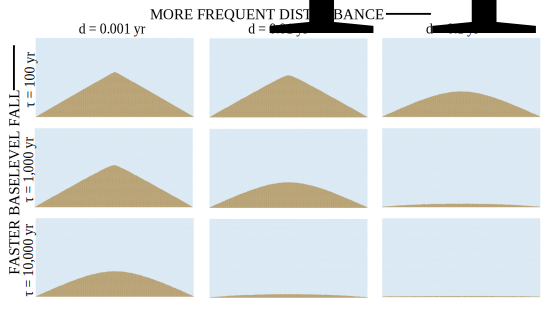
\includegraphics{Figures/simple_hills_3x3.pdf}
\caption{Equilibrium topographic cross-sections using only soil particles (no rock) and a variety of disturbance frequencies ($d$) and time interval between baselevel fall events ($\tau$). Fast basal incision and/or infrequent disturbance leads to planar threshold hillslopes; slow basal incision and/or frequent disturbance leads to parabolic hillslopes.}
\label{tlim}
\end{figure*}

Scaling of mean height as a function of $d'$ is shown in Figure~\ref{tlimscaling}. The figure shows results for 125 model runs spanning two orders of magnitude in each parameter ($d$, $\tau$, and $\lambda$) in half-decade intervals. For any given hillslope length, there are three regimes of behavior. Low $d'$ (upper left of graph) leads to threshold hillslopes, in which relief depends only on hillslope length. Under moderate $d'$, relief scales inversely with $d'$, as expected from linear diffusion theory. At high $d'$, we have a finite-size regime in which hillslope relief is comparable to the disturbance scale, $\delta$ (cell size in the model); in other words, the hill is only one or a few cells high.

%f
\begin{figure*}[t]
\includegraphics[width=8cm]{Figures/mean_ht_vs_dist_rate.pdf}
\caption{}
\label{tlimscaling}
\end{figure*}

The behavior of the grain hill model in its simple, transport-limited configuration can be compared to diffusion theory, which relates volumetric sediment flux per unit contour length to topographic gradient:
\begin{equation}
\mathbf{q}_s = -D \frac{\partial \eta}{\partial x}
\label{qs}
\end{equation}
where $\eta$ is land-surface height, $x$ is horizontal distance, and $D$ is an effective transport coefficient. The \citet{furbish2009statistical} probabilistic theory for transport due to particle scattering and settling formulates $D$ as
\begin{equation}
D = k R h \overline{N_a \left( 1 - \frac{c}{c_m}\right)^2} \cos^2 \theta
\end{equation}
where $k$ is a dimensionless coefficient, $R$ is particle radius, $h$ is active soil thickness, $N_a$ is the activation rate, $\theta$ is slope angle, $c$ is particle concentration, and $c_m$ is a maximum concentration. The over-bar denotes an average over the active soil thickness. For the grain hill model, $h$ scales with the characteristic disturbance depth, $\delta$. Further, because we treat grain aggregates, we may also assume $R\sim \delta$. Therefore, we have the prediction that
\begin{equation}
D = a \delta^2 N_a \cos^2 \theta
\label{D}
\end{equation}
where $a$ is a dimensionless proportionality constant.  

In the grain hill model, the mean expected activation rate, $N_a$, depends on gradient. On a flat surface, $N_a$ is equal to the mean disturbance rate, $d$. On a sloping surface that is gentler than the 30$^\circ$ effective angle of repose, $N_a$ has a weak dependence on gradient because the probability per time that a particle will be mobilized depends on the number of its six faces that are exposed to a fluid cell. At a gradient of exactly 30$^\circ$, two faces will be exposed. In this case, the random variable representing time to disturbance is the minimum of two exponentially distributed random variables (that is, the time to next disturbance at face 1, and the time at face 2). The distribution of the minimum of two independent exponential random variables with the same mean is itself exponential, with the expected value equal to half the original distribution's mean. Thus, with two faces exposed (at 30$^\circ$), the mean activation rate is $N_a = 2d$. Above 30$^\circ$, the rate increases dramatically because gravitational dislodgment is activated (Figure~\ref{gravity}, bottom row). Thus, the grain hill model incorporates an additional nonlinear relationship between flux and gradient inasmuch as $N_a$ depends on gradient.

We can derive an effective diffusivity, $D_e$, from the modeled topography by applying the expected relationship between mean elevation and diffusivity. Here $D_e$ is defined as that value which, if it were spatially uniform, would yield the same mean steady-state elevation as that produced by the particle model. Framing it this way allows us to interrogate how the effective transport coefficient varies as a function of mean slope gradient. At steady state, mass balance implies that
\begin{equation}
\mathbf{q}_s = E x
\end{equation}
where $E$ is the rate of erosion---equal to the rate of material uplift relative to baselevel---and $x$ is distance from the ridge top. Substituting equation (\ref{qs}) and rearranging,
\begin{equation}
\frac{d \eta}{d x} = -\frac{E}{D(x)} x \approx -\frac{E}{D_e} x
\end{equation}
Integrating and then averaging over $x$, we can solve for the average elevation, $\overline{\eta}$:
\begin{equation}
\overline{\eta} = \frac{E}{3 D_e} L^2
\end{equation}
where $L$ is the length of the slope from ridge top to base. We can then invert this to find $D_e$:
\begin{equation}
D_e = \frac{E}{3 \overline{\eta}} L^2
\end{equation}
To examine how $D_e$ scales, we can define a dimensionless form, normalizing by the disturbance frequency, $d$, and the square of active soil thickness (equal to particle diameter), $\delta^2$:
\begin{equation}
D_e' = \frac{D_e}{3 d\delta^2} = \frac{EL^2}{3\overline{\eta}d\delta^2}
\end{equation}
Noting that $E=\delta/\tau$ and $L/\delta = \lambda$, this is equivalent to
\begin{equation}
D_e' = \frac{\lambda^2}{3 \overline{h}d\tau}
\end{equation}
where $\overline{h}$ is the mean hillslope height in particle diameters.

As expected, $D_e'$ increases with hillslope gradient (Figure~\ref{diffgrad}). The effective diffusivity approaches an asymptote at 30$^\circ$, representing an angle of repose. The pattern resembles the family of nonlinear flux-gradient curves introduced by \citet{andrews} and explored further by \citet{howard1994detachment} and \citet{roering1999hillslope}. At low gradients, $D_e'$ approaches a value of about 10, which represents the product $a N_a(S\rightarrow 0)$ in equation (\ref{D}).

The link between $D_e$ and $d$ provides a way to scale the grain hill model to field-derived estimates of $D$ and $h$. Given the definition of $D_e' = \delta^2 d$ and the observation that $D_e' \approx 10$ at low gradient, an approximate equivalence between $d$ and $D$ is
\begin{equation}
D = 10 \delta^2 d.
\end{equation}
For example, if one were to assume an active soil thickness of 0.4~m and a low-gradient transport coefficient of $D = 0.01$~m$^2$/yr, and set $\delta$ to the active soil thickness, then
\begin{equation}
d = D \delta^{-2} = 0.0625 y^{-1}.
\end{equation}
With these values, the simulated hills in Figure~\ref{tlim} would be 232~m long with height ranging from 1.6 to 57.6~m.

%f
\begin{figure*}[t]
\includegraphics[width=8cm]{Figures/dimless_diff_vs_grad.pdf}
\caption{Relationship between dimensionless diffusivity and mean hillslope gradient, from the series of 125 model runs of which a subset are shown in Figure~\ref{tlim}.}
\label{diffgrad}
\end{figure*}


\subsection{Hillslope with regolith production from rock}

Having established that the grain hill model reproduces classic soil-mantled hillslope forms, we turn now to the case in which regolith is generated from bedrock with a production rate that may (or may not) limit the rate of erosion. We explore the role of regolith production with a series of model runs in which $w'$ varies from 0.4 to 40. This upper end of this range represents a condition in which the potential maximum rate of regolith production greatly exceeds the rate of baselevel lowering. The lower end, 0.4, is less than the rate of baselevel fall, and would seem to be insufficient to allow for equilibrium to occur, and yet nonetheless it does.

%f
\begin{figure*}[t]
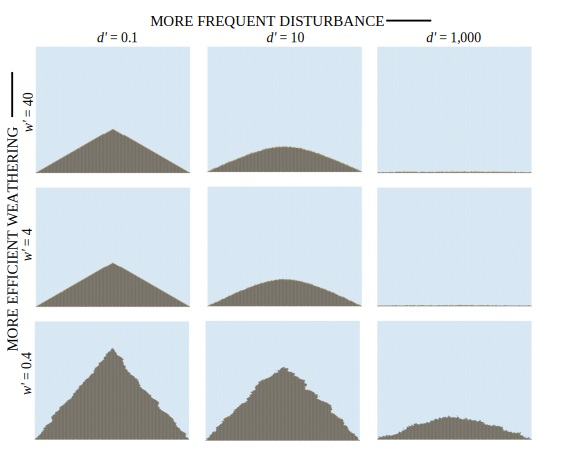
\includegraphics[width=8cm]{Figures/weathered_hills_3x3.pdf}
\caption{...}
\label{wxhills3x3}
\end{figure*}

Relationships among mean gradient, fractional soil cover, $d'$, and $w'$ are illustrated in Figure~\ref{wxing4x4}. For $w' > 1$, the gradient-$d'$ relation (Figure~\ref{wxing4x4}a) has the same pattern as in the purely soil models: a threshold regime at lower $d'$ transitioning to an inverse gradient-$d'$ relation at higher $d'$. This indicates that when the maximum weathering rate (for a flat surface) is substantially greater than the rate of baselevel fall, we recapture transport-limited conditions. With $w'<1$, however, the hillslope achieves an equilibrium gradient that is greater than that for the transport-limited case, and at lower $d'$, is greater than the threshold angle (Figures~\ref{wxing4x4}a,b).

We can also examine the fractional soil cover, which is defined here as the number of rock-air cell pairs divided by the total number cell pairs at which air meets either soil or rock (Figures~\ref{wxing4x4}c,d). The fractional soil cover shows relatively little sensitivity to $d'$ (Figure~\ref{wxing4x4}c). The cover approaches unity for high $w'$ and $d'$, but systematically declines with $w'$ when $w'$ is below about 10. (Note that the data points representing $d' = 1000$ and $w' > 1$ have hillslope heights of only a few particles, and therefore sensitive to finite-size effects).

%f
\begin{figure*}[t]
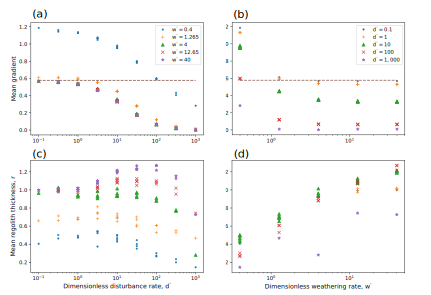
\includegraphics[width=12cm]{Figures/wxing_slope_frac_cover.pdf}
\caption{...}
\label{wxing4x4}
\end{figure*}

The models with $w' < 1$ present a seeming paradox: how is it possible to achieve an equilibrium form when the maximum weathering rate appears to be lower than the rate of uplift relative to baselevel? The solution to the paradox lies in surface area. The surface area of rock that is exposed to weathering is not fixed, but rather depends on the overall slope length, the terrain roughness, and the fractional soil cover. To appreciate the first effect, consider a planar slope at angle $\theta$ with no soil cover. If $w\delta$ represents the maximum slope-normal bedrock weathering rate, then the vertical rate is simply $w\delta / \cos \theta$. All else equal, increasing gradient will increase vertical weathering rate, thereby providing a feedback between gradient and rock lowering rate. A second feedback relates to topographic roughness: all else equal, a rougher surface will experience a greater weathering rate because it provides more surface area. The third feedback, which is embedded in the depth-dependent soil production hypothesis \citep{REFS} lies in soil cover: the greater the exposure of rock (or the thinner the cover), the faster the average rate of rock-to-soil conversion will be. In the grain hill model, this third feedback is represented by fractional bedrock exposure (since weathering only occurs when rock cells are juxtaposed with air cells).

To test whether these are indeed the feedbacks responsible for equilibrium topography in the grain hill model, we can compare the rate of material influx (uplift relative to baselevel) with the expected rate of rock-to-soil conversion. In the grain hill model, the expected rate of rock-to-soil conversion, $R$, in cross-sectional area per time, is the product of weathering rate per slope length, $w$, the width of a cell, $\delta$, and the total length of exposed rock, $\delta_f N_{ra}$,
\begin{equation}
R = w \delta \delta_f N_{ra},
\end{equation}
where $N_{ra}$ is the number of cell faces that juxtapose rock and air, and $\delta_f$ is the length of one face. The rate of material addition due to uplift relative to baselevel, $U$, again in cross-sectional area per time, is the height of a cell, $\delta$, times the horizontal width of the domain, $\lambda \delta$, divided by the interval between uplift events, $\tau$:
\begin{equation}
U = \delta^2 \lambda / \tau.
\end{equation}

%f
\begin{figure*}[t]
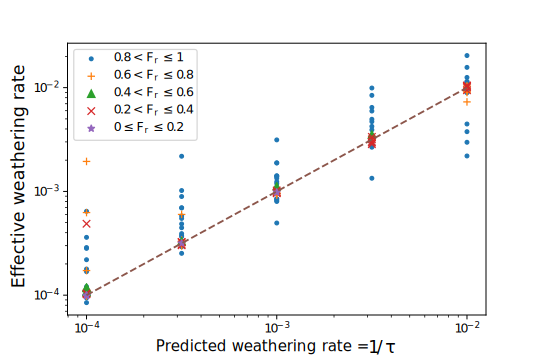
\includegraphics[width=12cm]{Figures/wxing_vs_uplift.pdf}
\caption{...}
\label{wxinguplift}
\end{figure*}




[FROM HERE: discuss seeming paradox that with a fixed particle weathering probability, model finds an equilibrium even when the weathering probability is lower than the uplift rate. how and why does that work? answer is that there is an additional feedback: the surface area of exposed rock. this is controlled by 3 things: the euclidean length of the hillslope, which is controlled by the mean gradient; the roughness of the surface; and the fractional soil cover. model must achieve an equilibrium in which the surface area times weathering rate equals the uplift rate times projected hillslope length. show plot indicating that it does indeed do this. probably save discussion of the extent to which this is a valid analogy for nature until the discussion.]

[... One feedback is about slope length: naively, with a planar slope that erodes at rate w in the slope normal direction, the vertical lowering rate would be w / cos theta. So at equilibrium with erosion rate E, cos theta = w / E, when w < E]




\subsection{Rock collapse}



[NEXT UP: EXPERIMENTS WITH WEATHERING!]









Ok, so what cases do we consider?

1 - soil-only hillslopes

2 - rocky hillslopes

3 - heavy particles


\section{Discussion}


\conclusions  %% \conclusions[modified heading if necessary]
TEXT




%\appendix


\authorcontribution{TEXT}

\begin{acknowledgements}
TEXT
\end{acknowledgements}


%% REFERENCES

%% The reference list is compiled as follows:

\bibliographystyle{copernicus}
\bibliography{/Users/gtucker/Documents/Literature/gt_library.bib}

%\begin{thebibliography}{}

%\bibitem[AUTHOR(YEAR)]{LABEL}
%REFERENCE 1

%\bibitem[AUTHOR(YEAR)]{LABEL}
%REFERENCE 2

%\end{thebibliography}

%% Since the Copernicus LaTeX package includes the BibTeX style file copernicus.bst,
%% authors experienced with BibTeX only have to include the following two lines:
%%
%% \bibliographystyle{copernicus}
%% \bibliography{example.bib}
%%
%% URLs and DOIs can be entered in your BibTeX file as:
%%
%% URL = {http://www.xyz.org/~jones/idx_g.htm}
%% DOI = {10.5194/xyz}


%% LITERATURE CITATIONS
%%
%% command                        & example result
%% \citet{jones90}|               & Jones et al. (1990)
%% \citep{jones90}|               & (Jones et al., 1990)
%% \citep{jones90,jones93}|       & (Jones et al., 1990, 1993)
%% \citep[p.~32]{jones90}|        & (Jones et al., 1990, p.~32)
%% \citep[e.g.,][]{jones90}|      & (e.g., Jones et al., 1990)
%% \citep[e.g.,][p.~32]{jones90}| & (e.g., Jones et al., 1990, p.~32)
%% \citeauthor{jones90}|          & Jones et al.
%% \citeyear{jones90}|            & 1990



%% FIGURES

%% ONE-COLUMN FIGURES

%%f
%\begin{figure}[t]
%\includegraphics[width=8.3cm]{FILE NAME}
%\caption{TEXT}
%\end{figure}
%
%%% TWO-COLUMN FIGURES
%
%%f
%\begin{figure*}[t]
%\includegraphics[width=12cm]{FILE NAME}
%\caption{TEXT}
%\end{figure*}
%
%
%%% TABLES
%%%
%%% The different columns must be seperated with a & command and should
%%% end with \\ to identify the column brake.
%
%%% ONE-COLUMN TABLE
%
%%t
%\begin{table}[t]
%\caption{TEXT}
%\begin{tabular}{column = lcr}
%\tophline
%
%\middlehline
%
%\bottomhline
%\end{tabular}
%\belowtable{} % Table Footnotes
%\end{table}
%
%%% TWO-COLUMN TABLE
%
%%t
%\begin{table*}[t]
%\caption{TEXT}
%\begin{tabular}{column = lcr}
%\tophline
%
%\middlehline
%
%\bottomhline
%\end{tabular}
%\belowtable{} % Table Footnotes
%\end{table*}
%
%
%%% NUMBERING OF FIGURES AND TABLES
%%%
%%% If figures and tables must be numbered 1a, 1b, etc. the following command
%%% should be inserted before the begin{} command.
%
%\addtocounter{figure}{-1}\renewcommand{\thefigure}{\arabic{figure}a}
%
%
%%% MATHEMATICAL EXPRESSIONS
%
%%% All papers typeset by Copernicus Publications follow the math typesetting regulations
%%% given by the IUPAC Green Book (IUPAC: Quantities, Units and Symbols in Physical Chemistry,
%%% 2nd Edn., Blackwell Science, available at: http://old.iupac.org/publications/books/gbook/green_book_2ed.pdf, 1993).
%%%
%%% Physical quantities/variables are typeset in italic font (t for time, T for Temperature)
%%% Indices which are not defined are typeset in italic font (x, y, z, a, b, c)
%%% Items/objects which are defined are typeset in roman font (Car A, Car B)
%%% Descriptions/specifications which are defined by itself are typeset in roman font (abs, rel, ref, tot, net, ice)
%%% Abbreviations from 2 letters are typeset in roman font (RH, LAI)
%%% Vectors are identified in bold italic font using \vec{x}
%%% Matrices are identified in bold roman font
%%% Multiplication signs are typeset using the LaTeX commands \times (for vector products, grids, and exponential notations) or \cdot
%%% The character * should not be applied as mutliplication sign
%
%
%%% EQUATIONS
%
%%% Single-row equation
%
%\begin{equation}
%
%\end{equation}
%
%%% Multiline equation
%
%\begin{align}
%& 3 + 5 = 8\\
%& 3 + 5 = 8\\
%& 3 + 5 = 8
%\end{align}
%
%
%%% MATRICES
%
%\begin{matrix}
%x & y & z\\
%x & y & z\\
%x & y & z\\
%\end{matrix}
%
%
%%% ALGORITHM
%
%\begin{algorithm}
%\caption{�}
%\label{a1}
%\begin{algorithmic}
%�
%\end{algorithmic}
%\end{algorithm}
%
%
%%% CHEMICAL FORMULAS AND REACTIONS
%
%%% For formulas embedded in the text, please use \chem{}
%
%%% The reaction environment creates labels including the letter R, i.e. (R1), (R2), etc.
%
%\begin{reaction}
%%% \rightarrow should be used for normal (one-way) chemical reactions
%%% \rightleftharpoons should be used for equilibria
%%% \leftrightarrow should be used for resonance structures
%\end{reaction}
%
%
%%% PHYSICAL UNITS
%%%
%%% Please use \unit{} and apply the exponential notation


\section{Background}

Do we go all the way back to Gilbert? probably, but quite briefly. 

gilbert reasoned that the rate of release of rock or saprolite to disaggregated material should depend on the thickness of the overlying regolith cover, because XYZ. this was later codified into the popular inverse-exponential and ``humped curve'' formulas [ahnert, heimsath, anderson, etc]. consistent with cosmo nuclides [heim, small, etc]. lacks mechanistic basis.

Davis and Gilbert enunciated the view of convex soil-mantled slopes, turned into math by culling, who also nodded to underlying probabilistic basis.

diffusion theory captures convex slopes, and is consistent with cosmos [mckean, small, ...]

modified to account for accelerated motion, nonlinear, andrews and bucknam, howard, roering

also modified for account for depth dependence

process blind; some specific formulations for particular types of disturbance process (e.g., frost creep) (just mentioning in passing)

Furbish work that relates bulk flux of sediment to the statistical mechanics of grain motion, leading to diffusion-like principles. Foufoula nonlocal and fractional calculus.

hillslope cellular and particle models review: jyotsna and haff, tucker and bradley, roering and ?.

meanwhile, in the granular mechanics community, a whole variety of cellular models (see refs in T et al 2016)

one of our aims in this paper is to forge a link between the lattice-grain models used in the granular mechanics community, and theories for hillslope evolution in the geomorphology community.



\end{document}
